\chapter{Implementação}
\label{implementation-algorithm}

Neste capítulo será apresentado detalhes da implementação deste trabalho. Será apresentado a arquitetura que foi criada para o desenvolvimento do algoritmo proposto, um diagrama de sequência, que proverá uma visibilidade sobre os passos que são seguidos na execução do algoritmo e uma explicação sobre os elementos que compõe o algoritmo.

\section{Arquitetura}

A figura \ref{architecture} demonstra a arquitetura que foi utilizada para a realização dos experimentos. A arquitetura foi desenvolvida afim de se aproximar a uma utilização real de um algoritmo de criptografia. As partes do cifrador e do decifrador são utilizadas em dois computadores distintos utilizando o protocolo de rede TCP/IP.

De maneira geral, cada lado terá uma \textit{thread} que auxiliará no envio do \textit{byte} cifrado usando o \textit{socket} TCP/IP. A parte de cifração/decifração será utilizando o núcleo do \textit{RC4} e junto utilizando o algoritmo proposto.

\begin{figure}[h]
	\centering
	\includegraphics[scale=0.5]{figuras/architecture.eps}
	\caption{Arquitetura utilizada no projeto}
	\label{architecture}
\end{figure}

\subsection{Inicializador do Gerador}

Esse elemento é responsável por fazer a inicialização do gerador que será utilizado  no algoritmo.

O gerador escolhido para os experimentos foi o do próprio \textit{RC4}. A entrada utilizada é uma chave gerada pelo \textit{ssh-keygen}.

\subsection{Gerador de \textit{Bytes}}

Como explicado anteriormente, o gerador escolhido foi o do próprio \textit{RC4} e sua geração foi feita de acordo com que o algoritmo aconselha. 


\subsection{Fila de Mensagem}

A fila de mensagem foi utilizada para intermediar entre o cifrador/decifrador e a \textit{thread} que enviaria/receberia os \textit{bytes}. 

Primeiramente, o cifrado escreve os \textit{bytes} cifrados na fila de mensagem. A \textit{thread} é responsável por realizar a leitura dos \textit{bytes} e envia-los para o decifrador.

No decifrador, por sua vez, a \textit{thread} é responsável por receber os \textit{bytes} que são enviados pelo cifrador e escreve-las na fila de mensagem do decifrador. O decifrador realiza as operações a partir dos \textit{bytes} que estão contidos na fila de mensagem.
  
\subsection{\textit{Thread} de Envio para Decifrador}

No processo de cifração, para auxiliar o envio dos \textit{bytes} cifrados, é utilizado uma \textit{thread} que sua responsabilidade é fazer a leitura da fila de mensagem e enviar os \textit{bytes} ali contidos. 

Isso foi feito, pois a comunicação é a parte que mais causará \textit{overhead} no algoritmo e para fazer com que a execução não fosse atrapalhada pela troca de mensagens entre os processos.
\subsection{\textit{Thread} para Receber do Cifrador}

Assim como no cifrador, o decifrador também conta com uma \textit{thread} auxiliadora para receber os \textit{bytes} que são enviados pelo cifrador e escrever na fila de mensagem.

\subsection{\textit{TCP/IP}}

Quando estávamos analisando o melhor protocolo de comunicação para ser utilizado em conjunto com o algoritmo, decidimos pelo TCP/IP pela reciprocidade que o mesmo contém. 

Em algoritmos de criptografia, a ordem com que os \textit{bytes} são enviados/lidos é de extrema importância, para que o texto decifrado tenha consistência e integridade. 
\subsection{Decifrador}

Processo responsável em fazer a tradução dos \textit{bytes} cifrados. 

O decifrador irá ter acesso aos \textit{bytes} cifrados na fila de mensagem que será populada pela \textit{thread} de recebimento. A operação que é efetuada é somente um ou-exclusivo do \textit{byte} proveniente do gerador e o \textit{byte} correspondente.

\subsection{Cifrador}

Processo responsável em cifrar os \textit{bytes} em claro que se deseja obter segurança.

O cifrador fará a leitura dos \textit{bytes} em claro de um arquivo e fará a operação ou-exclusivo com o \textit{byte} d gerador.

\section{Diagrama de Sequência}

O diagrama de sequência representado na figura \ref{sequence-diagram} tem como objetivo demonstrar como os processos,cifra e  decifra, interagem com os outros elementos, tais como: fila de mensagem, \textit{threads} e a comunicação entre os mesmos. 

\begin{figure}[h]
	\centering
	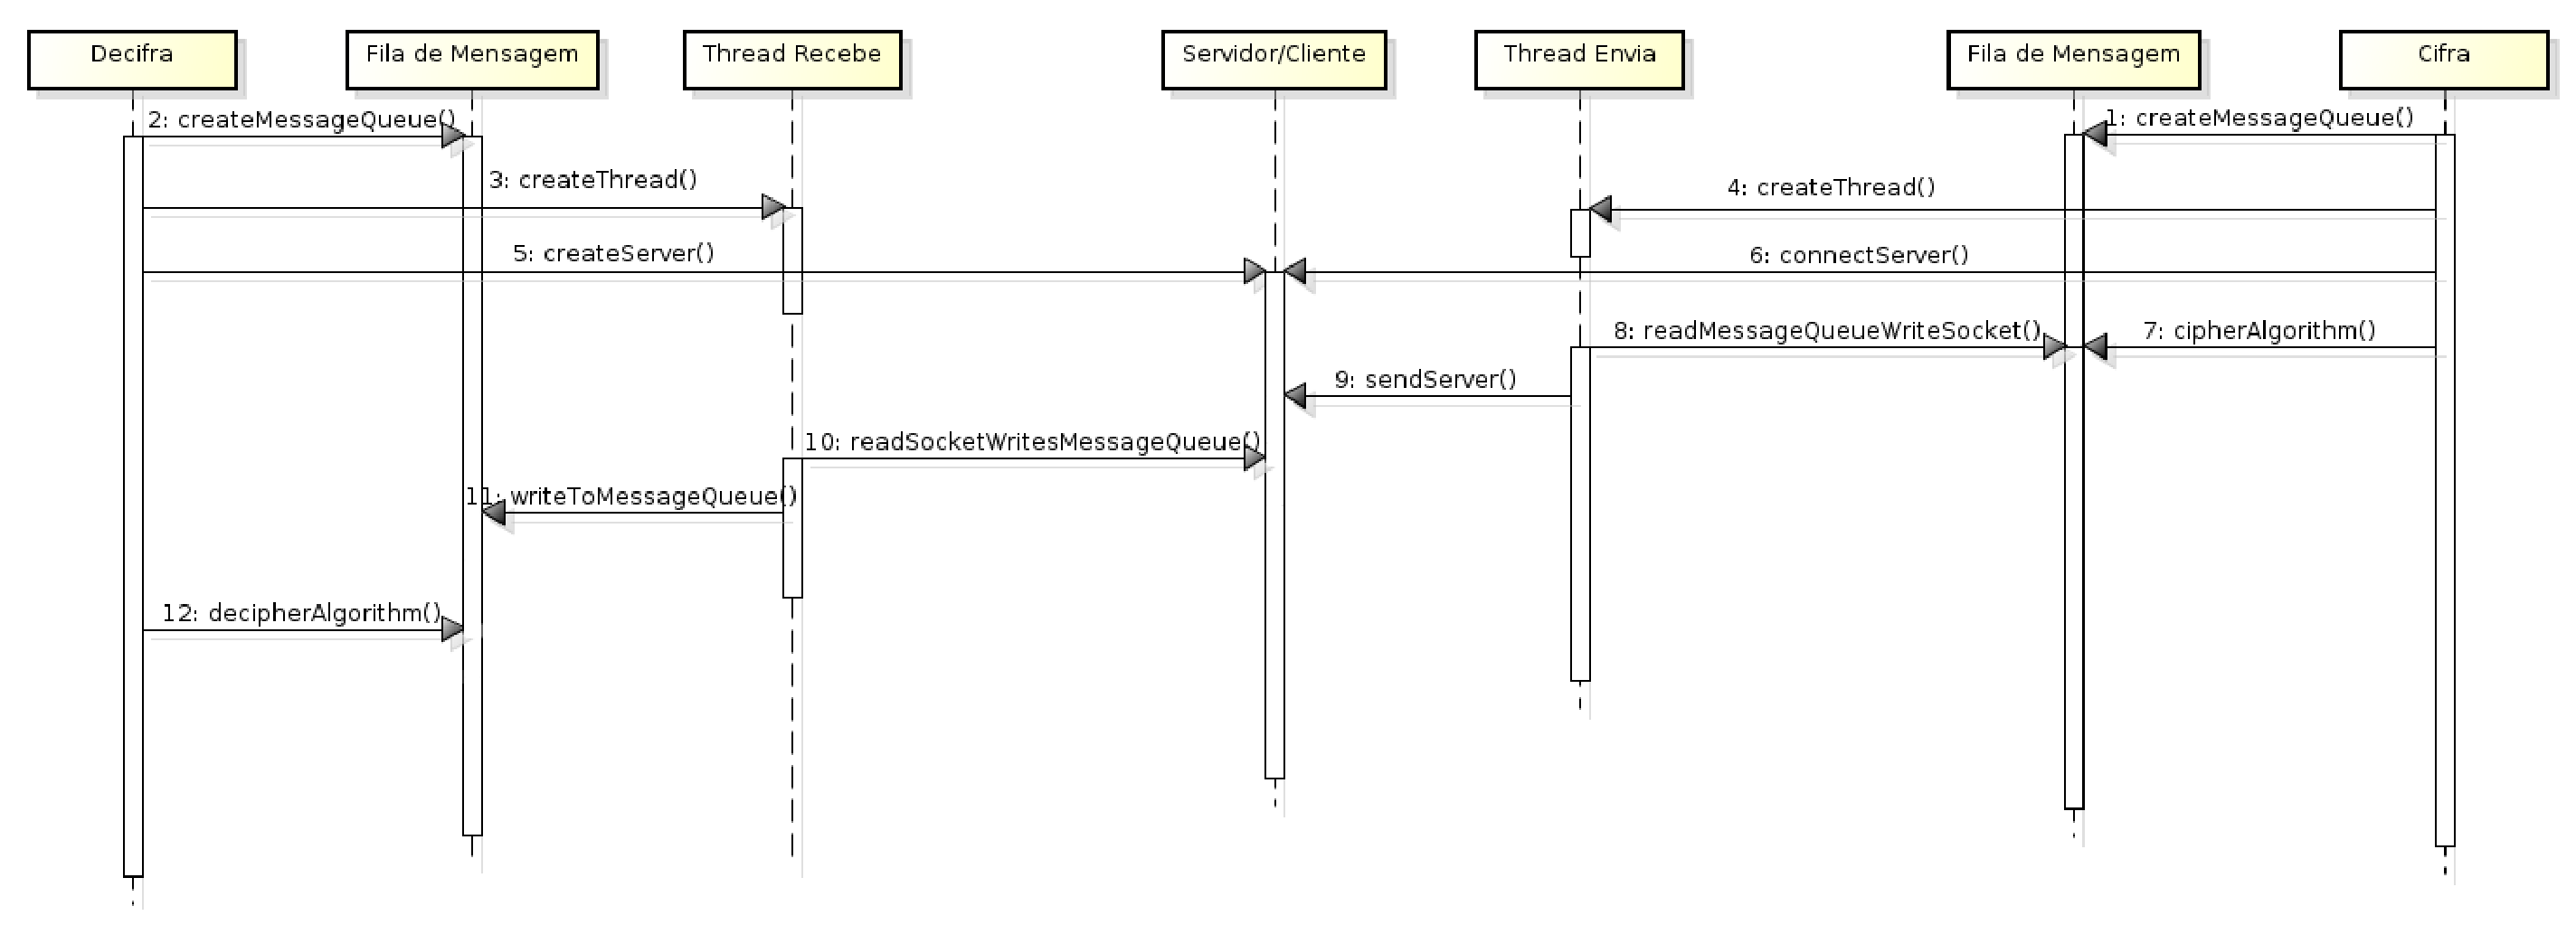
\includegraphics[scale=0.5, angle = 90]{figuras/sequenceDiagram.eps}
	\caption{Diagrama de Sequência}
	\label{sequence-diagram}
\end{figure}

O primeiro processo que deve ser iniciado é o de decifração, ele é responsável por iniciar o servidor em que o processo de cifra irá se conectar para fazer a comunicação e envio de \textit{bytes} cifrados. Como apresentado na arquitetura, cada lado da comunicação tem uma \textit{thread} para auxiliar os processos e uma fila de mensagem para fazer o intermédio entre o processo e essa \textit{thread}. No lado da decifração, o objetivo da \textit{thread} é fazer a leitura do \textit{socket} de comunicação e escrever as mensagens obtidas nessa leitura na fila de mensagem. O processo de decifração irá fazer a leitura dessa fila de mensagem para realizar a decifração.

Quando o processo de cifração é iniciado é preciso realizar a conexão com o servidor e o servidor precisa aceita-lo. Ao fazer essa conexão, o processo de cifração está pronto para fazer a comunicação, portanto, é necessário iniciar os elementos auxiliares, como a \textit{thread} que irá fazer a leitura da fila de mensagem e enviar para o lado do decifrador e também a própria fila de mensagem. Então, primeiramente o processo de cifração faz a leitura do arquivo que contém a mensagem a ser cifrada e realiza a cifração. Após a cifração, essa mensagem é colocada na fila de mensagem e a partir daí a \textit{thread} é responsável de enviar essa mensagem para o lado do servidor.